



	
	\begin{center}
		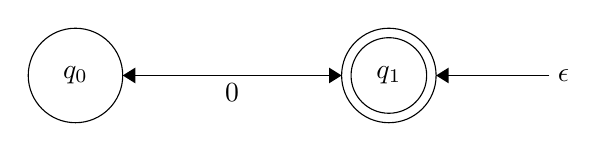
\begin{tikzpicture}[scale=0.2]
		\tikzstyle{every node}+=[inner sep=0pt]
		\draw [black] (40.6,-19.3) circle (3);
		\draw (40.6,-19.3) node {$q_1$};
		\draw [black] (40.6,-19.3) circle (2.4);
		\draw [black] (20.7,-19.3) circle (3);
		\draw (20.7,-19.3) node {$q_0$};
		\draw [black] (37.6,-19.3) -- (23.7,-19.3);
		\fill [black] (23.7,-19.3) -- (24.5,-19.8) -- (24.5,-18.8);
		\draw [black] (23.7,-19.3) -- (37.6,-19.3);
		\fill [black] (37.6,-19.3) -- (36.8,-18.8) -- (36.8,-19.8);
		\draw (30.65,-19.8) node [below] {$0$};
		\draw [black] (50.8,-19.3) -- (43.6,-19.3);
		\draw (51.3,-19.3) node [right] {$\epsilon$};
		\fill [black] (43.6,-19.3) -- (44.4,-19.8) -- (44.4,-18.8);
		\end{tikzpicture}
	\end{center}
	
